\section{Results} \label{sec:results}
For our second experiment we ran the methods detailed in the previous section on Ubuntu Linux server with 4 Intel(R) Xeon(R) CPU E5-2630 v3 @ 2.40GHz processors and 30GB of RAM.  In Tables \ref{tab:performance-runtime} and \ref{tab:performance-latency} we can see the results of running all three approaches in terms of required computation time and in terms of the average latency of the networks produced. Looking at just the performance data for the Naive and Greedy approach we see two clear trends.


First, we see that the runtime complexity of the Naive approach is very poor. In fact, networks of size $N>7$ were effectively not computable after 1 hour of computation time. In our experiment we decided to limit the runtime of any one algorithm to one hour because the cost model of many cloud providers is based on hourly billing. Any for a very large network, running more than an hour will cause a user to incur unnecessary cost. The second observation is that the naive approach is always better than the greedy approach in terms of latency for $N \leq 7$, but the Naive approach is not viable beyond that point. As the network size increases, the greedy approach finds better and better networks while keeping well within acceptable computation limits.   




In terms of achieving the goal function, both the naive and greedy approaches meet the objective latency of $0.5$ms, however, the greedy approach only achieves this for networks larger than 5 whereas for all networks the naive approach computed this value is reached every time. 

Next we will look at the results of our machine learning experiment. 

While the greedy classifier performs more optimally in terms of runtime, the decision tree classifier outperforms the greedy classifier and only performs slightly worse than the naive approach (a mater of thousands of a second in most cases).

Aside from the performance of the decision tree classifier, a few other points are of note. First, our approach relies on getting positive predictions from the classifier to consider it as a candidate node for a network. In our case, with our limited sample size, for networks larger than 20 nodes there were sometimes not enough nodes predicted to be in the correct class. In these cases we pick a node at random and insert it into the network. In future this effect could be mitigated by selecting a larger population to sample. We also believe that this limitation is what creates the spies in latency at $N=20$ and $N=50$


\begin{table}
  \caption{Runtime performance of the three approaches. Note for $N > 6$ the naive approach did not complete in a reasonable amount of time and thus the data is considered missing.}

  \centering
  \begin{tabular}{| c || c | c | c |}
    \hline 
    N & Naive & Greedy &  Decision Tree  \\
    \hline
    2 &  0.0003           &  0.0002      &  0.003  \\
    \hline
    3 &  0.008           &  0.0006      &   0.008\\
    \hline
    4 &  0.103          &  0.0011      &   0.212\\
    \hline
    5 &  0.102         &  0.0019      &   0.029\\
    \hline
    6 &  92.78       &  0.0027       &   0.049\\
    \hline
    7 &  2077.93              &  0.0036       &  0.065 \\
    \hline
    10 &  -             &  0.0071      &   0.13\\
    \hline
    20 &   -            &  0.0353      &   0.53 \\
    \hline
    50 &   -            &  0.3118      &   3.27\\
    \hline

  \end{tabular}
  \label{tab:performance-runtime}
\end{table}

\begin{table}
  \caption{Average network latency for networks generated from each of the three approaches. Note for $N > 6$ the naive approach did not complete in a reasonable amount of time and thus the data is considered missing.}

  \centering
  \begin{tabular}{| c || c | c | c |}
    \hline 
    N & Naive & Greedy & Decision Tree  \\
    \hline
    2 &  .3942     &   .522     &  .456 \\
    \hline
    3 &  .405       &   .507     & .495  \\
    \hline
    4 &  .471       &   .510     & .485  \\
    \hline
    5 &  .499       &   .501     & .483  \\
    \hline
    6 &  .497      &   .494     &  .475 \\
    \hline
    7 &  .491           &   .497     & .466  \\
    \hline
    10 &  -          &   .495     &  .461 \\
    \hline
    20 &   -         &   .497     &  .815 \\
    \hline
    50 &   -         &   .498     &  .581 \\
    \hline

  \end{tabular}
  \label{tab:performance-latency}
\end{table}


\begin{figure*}[ht]
\begin{subfigure}{0.48\textwidth}
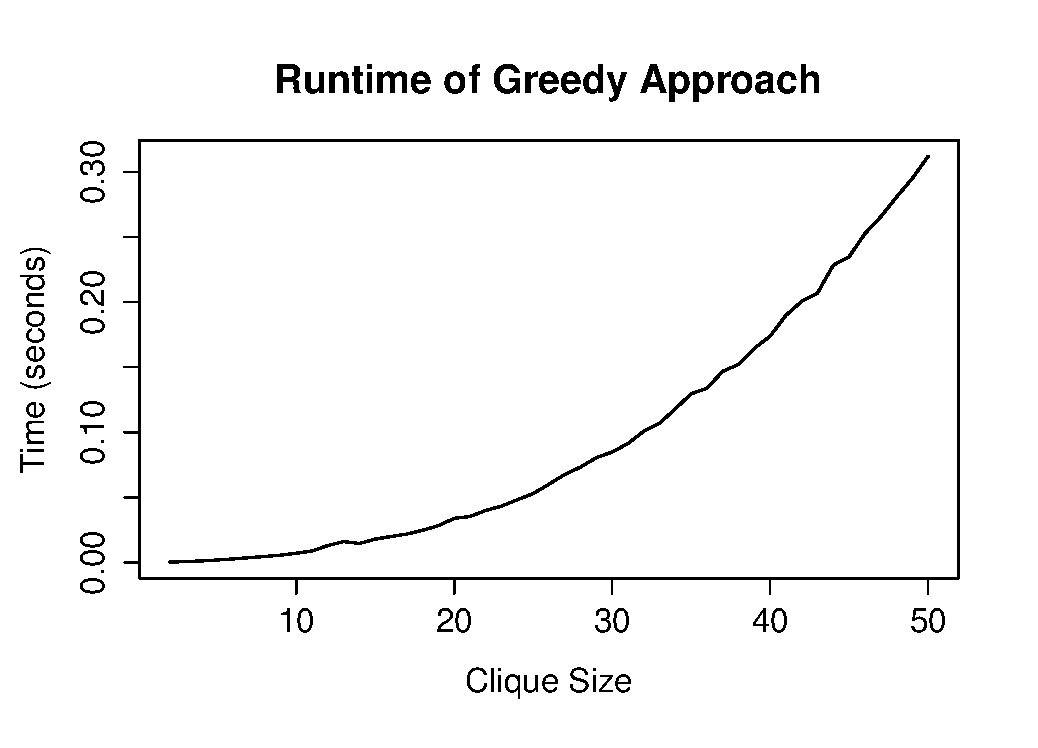
\includegraphics[width=\linewidth]{figures/greedy-runtime}
\caption{Runtime performance of the greedy approach on Cliques sizes from $N=2$ to $N=50$.}
\label{fig:greedy-runtime}
\end{subfigure}\hspace*{\fill}
\begin{subfigure}{0.48\textwidth}
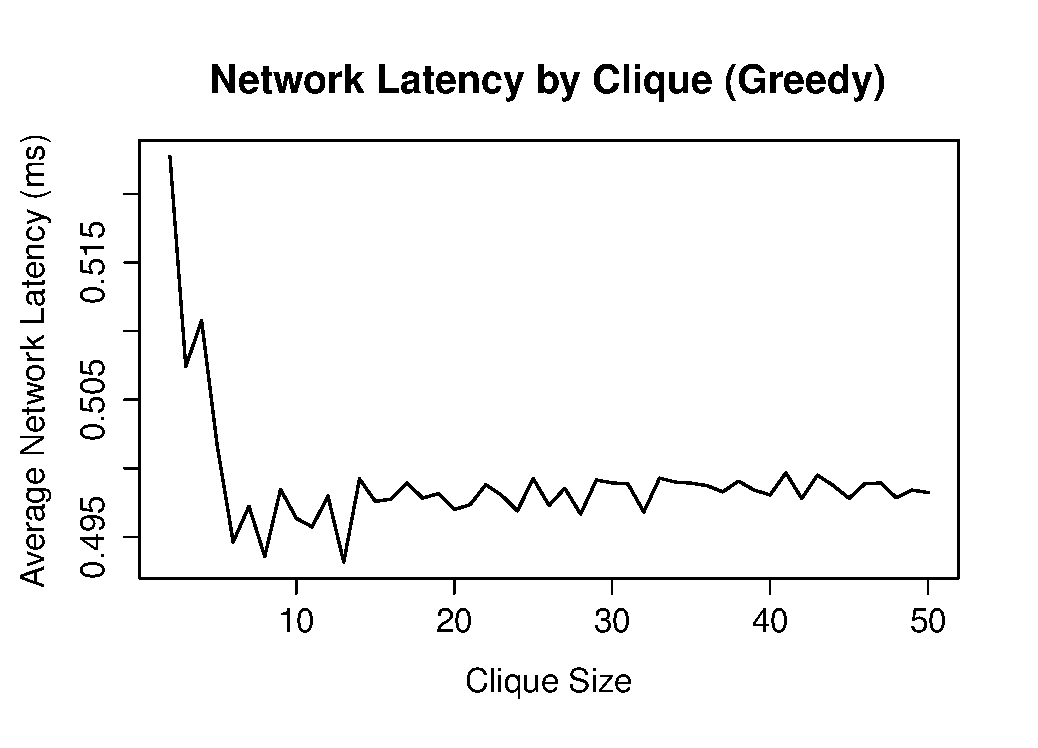
\includegraphics[width=\linewidth]{figures/greedy-latency}
\caption{Average latency of networks formed from the greedy approach on Cliques sizes from $N=2$ to $N=50$.}
\label{fig:greedy-latency}
\end{subfigure}
\end{figure*}


\medskip
\begin{figure*}[ht]
\begin{subfigure}{0.48\textwidth}
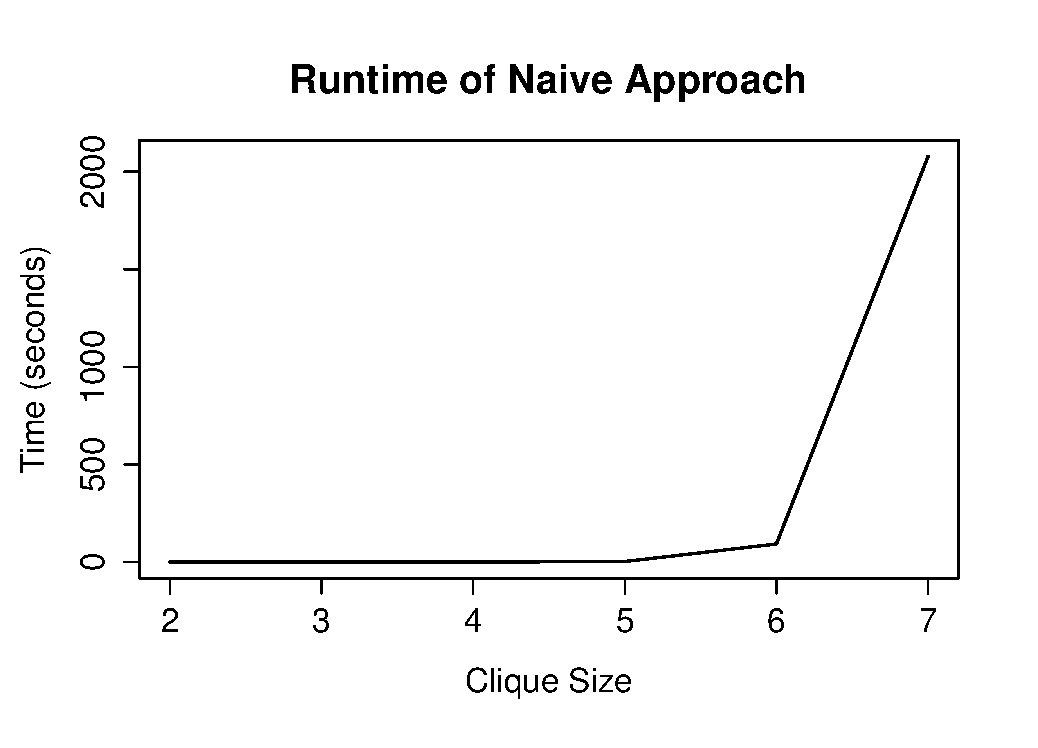
\includegraphics[width=\linewidth]{figures/naive-runtime}
\caption{Runtime performance of the naive approach on Cliques sizes from $N=2$ to $N=7$.}
\label{fig:naive-runtime}
\end{subfigure}\hspace*{\fill}
\begin{subfigure}{0.48\textwidth}
\includegraphics[width=\linewidth]{figures/naive-latency}
\caption{Average latency of networks formed from the naive approach on Cliques sizes from $N=2$ to $N=7$.}
\label{fig:naive-latency}
\end{subfigure}
\end{figure*}

\medskip
\begin{figure*}[ht]
\begin{subfigure}{0.48\textwidth}
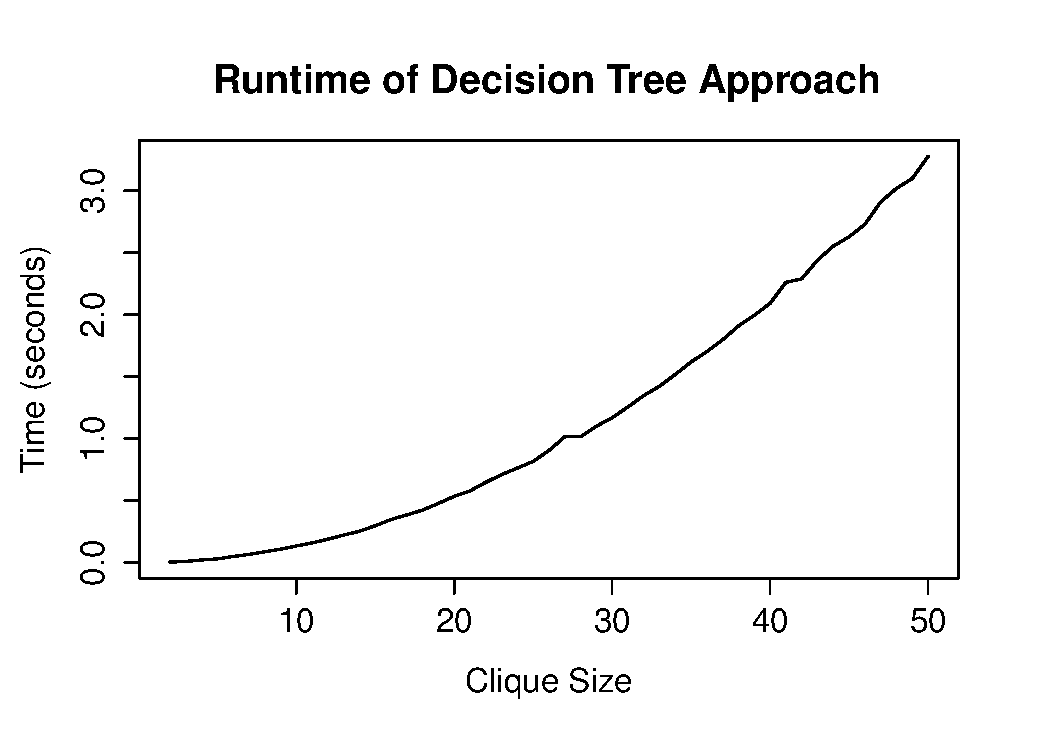
\includegraphics[width=\linewidth]{figures/decisiontree-runtime}
\caption{Runtime performance of the decision tree approach on Cliques sizes from $N=2$ to $N=50$.}
\label{fig:decisiontree-runtime}
\end{subfigure}\hspace*{\fill}
\begin{subfigure}{0.48\textwidth}
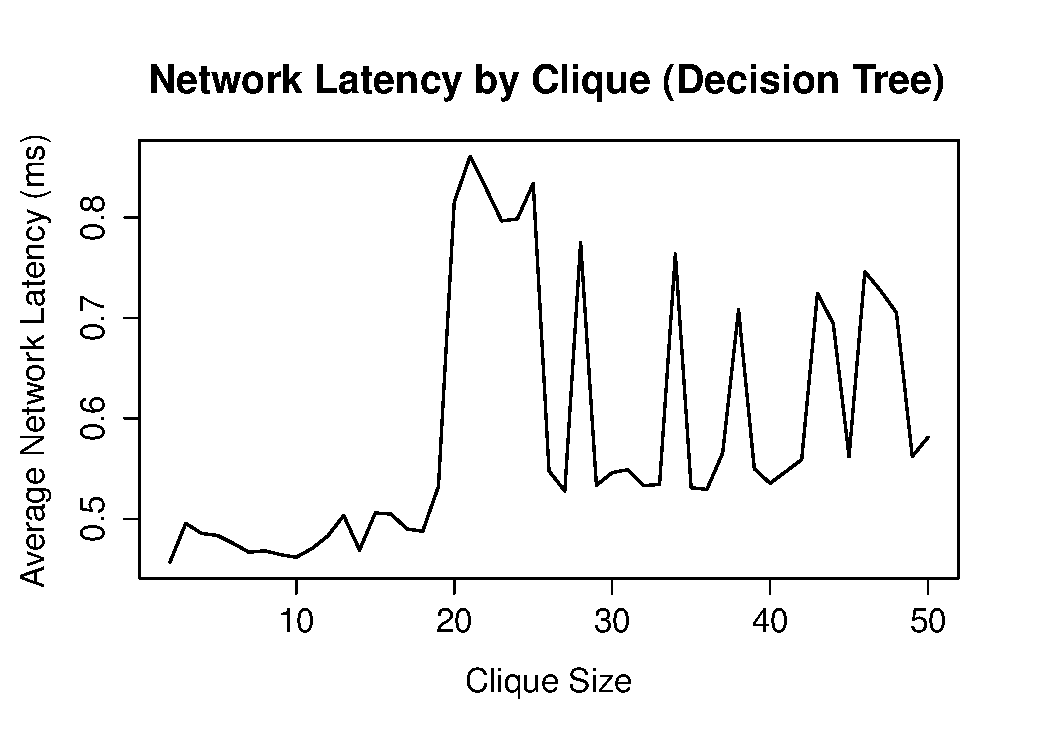
\includegraphics[width=\linewidth]{figures/decisiontree-latency}
\caption{Average latency of networks formed from the decision tree approach on Cliques sizes from $N=2$ to $N=50$.}
\label{fig:decisiontree-latency}
\end{subfigure}
\caption{ Hey John! Please write a comprehensive caption for this set of graphs here} \label{fig:1}
\end{figure*}


%\begin{figure*}[ht]
%  \centering 
%  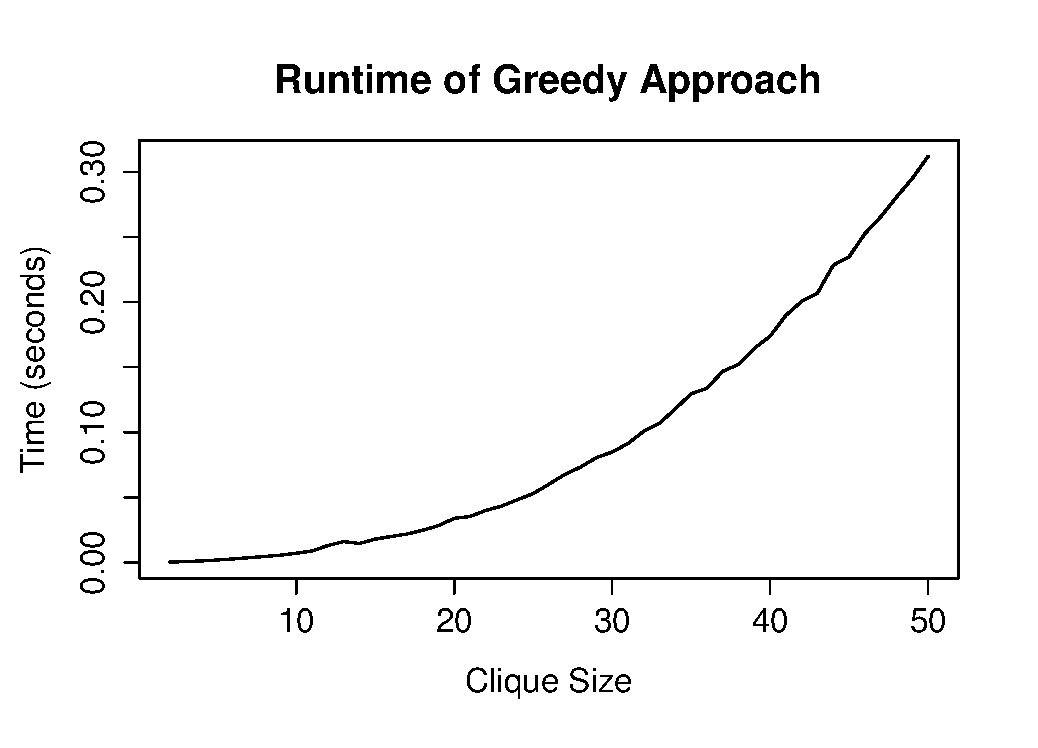
\includegraphics[scale=.8]{figures/greedy-runtime}
%  \caption{Runtime performance of the greedy approach on Cliques sizes from $N=2$ to $N=50$.}
%  \label{fig:greedy-runtime}
%\end{figure*}
%
%
%\begin{figure*}[ht]
%  \centering
%  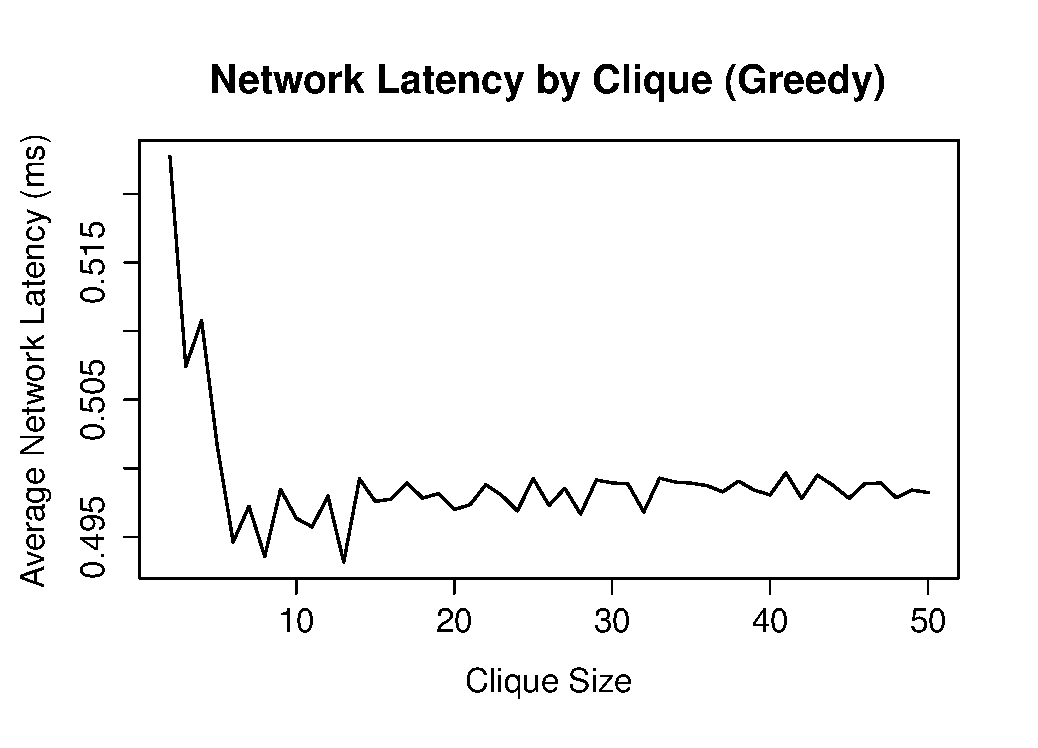
\includegraphics[scale=.8]{figures/greedy-latency}
%  \caption{Average latency of networks formed from the greedy approach on Cliques sizes from $N=2$ to $N=50$.}
%  \label{fig:greedy-latency}
%\end{figure*}
%
%\begin{figure*}[ht]
%  \centering 
%  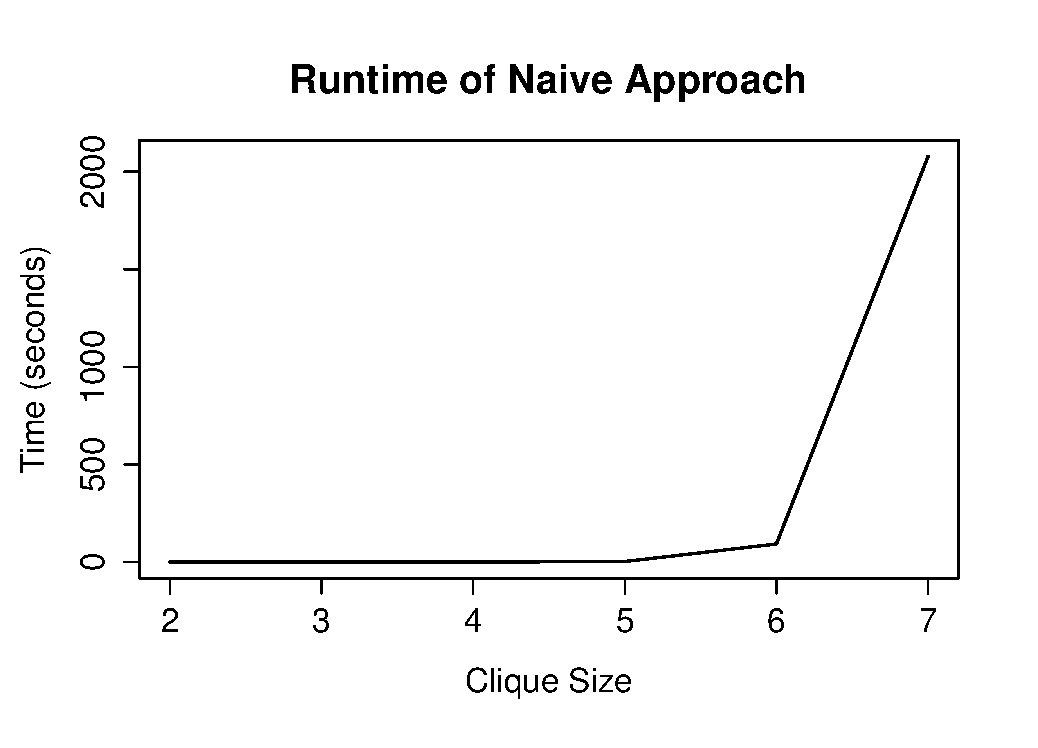
\includegraphics[scale=.8]{figures/naive-runtime}
%  \caption{Runtime performance of the naive approach on Cliques sizes from $N=2$ to $N=7$.}
%  \label{fig:naive-runtime}
%\end{figure*}
%
%
%\begin{figure*}[ht]
%  \centering
%  \includegraphics[scale=.8]{figures/naive-latency}
%  \caption{Average latency of networks formed from the naive approach on Cliques sizes from $N=2$ to $N=7$.}
%  \label{fig:naive-latency}
%\end{figure*}
%
%
%
%\begin{figure*}[ht]
%  \centering 
%  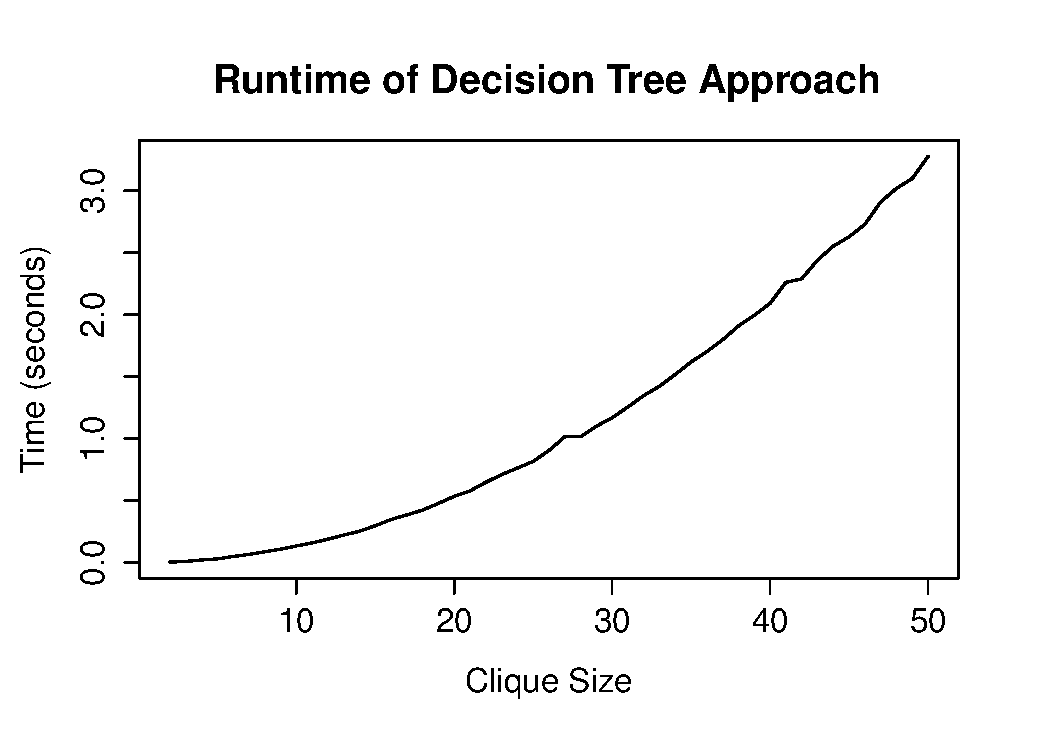
\includegraphics[scale=.8]{figures/decisiontree-runtime}
%  \caption{Runtime performance of the decision tree approach on Cliques sizes from $N=2$ to $N=50$.}
%  \label{fig:decisiontree-runtime}
%\end{figure*}
%
%
%\begin{figure*}[ht]
%  \centering
%  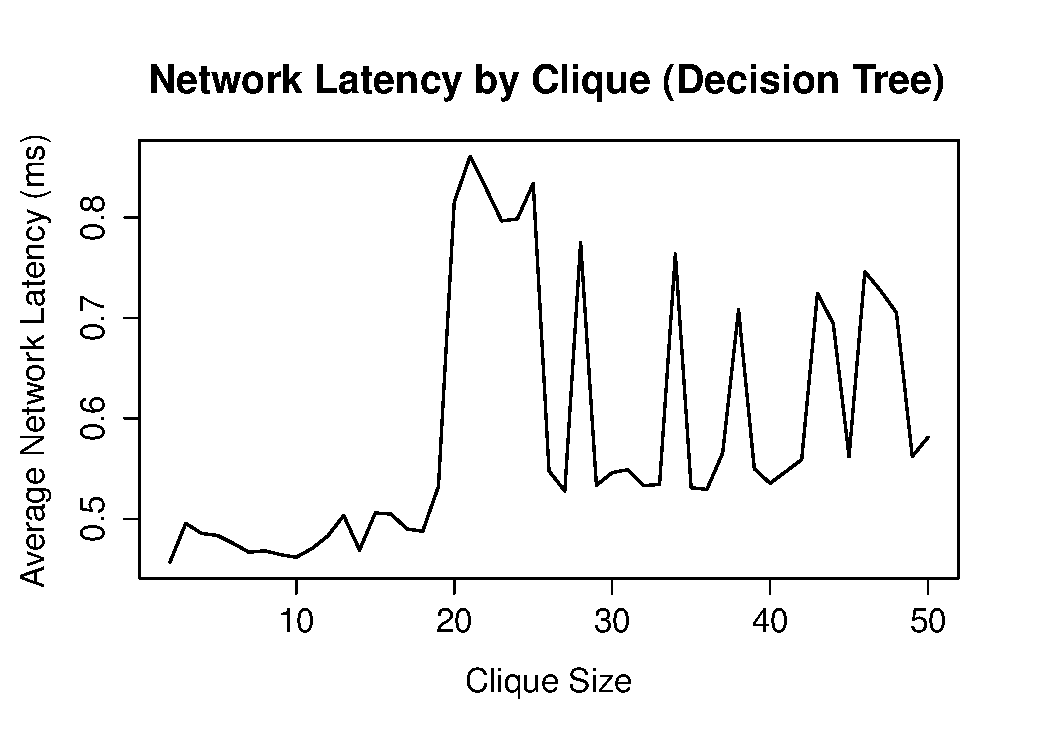
\includegraphics[scale=.8]{figures/decisiontree-latency}
%  \caption{Average latency of networks formed from the decision tree approach on Cliques sizes from $N=2$ to $N=50$.}
%  \label{fig:decisiontree-latency}
%\end{figure*}


%%% Local Variables:
%%% mode: latex
%%% TeX-master: "IPDPS2017"
%%% End: